% flashcards-title: Measured cup-stack heights with two competing model lines
% flashcards-desc: Axes with number of cups across and stack height in centimeters up. Three measured points sit at two cups eleven centimeters, four cups thirteen centimeters, and six cups fifteen centimeters. A dashed line labeled model A rises from the origin. A solid line labeled model B starts near nine centimeters on the height axis and rises gently through the region of the points.
\documentclass[dvisvgm,tikz,border=8pt]{standalone}
\usepackage{tikz}
\usetikzlibrary{arrows.meta,calc,positioning}
\definecolor{DeckInk}{HTML}{172A3A}
\definecolor{DeckAccent}{HTML}{176B87}
\definecolor{DeckWarm}{HTML}{D97706}
\definecolor{DeckMuted}{HTML}{667784}
\definecolor{DeckPaper}{HTML}{F7FAFC}
\tikzset{
  every node/.style={font=\sffamily, text=DeckInk},
  object/.style={draw=DeckInk, line width=1.1pt, fill=DeckPaper},
  primary/.style={draw=DeckAccent, line width=1.5pt},
  boundary/.style={draw=DeckAccent, line width=1.5pt, dashed, rounded corners=6pt},
  guide/.style={draw=DeckMuted, line width=0.9pt, dashed},
  dimension/.style={{Stealth[length=3.2mm,width=2.2mm]}-{Stealth[length=3.2mm,width=2.2mm]}, draw=DeckWarm, line width=1.2pt},
  motion/.style={-{Stealth[length=3.5mm,width=2.5mm]}, draw=DeckAccent, line width=1.5pt, dashed},
}

\begin{document}
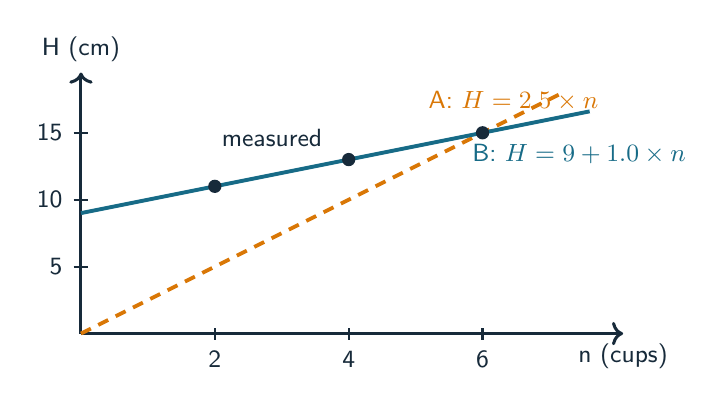
\begin{tikzpicture}[x=0.85cm, y=0.17cm]
  % Axes
  \draw[object, ->] (0,0) -- (8.1,0) node[below, font=\sffamily\small] {n (cups)};
  \draw[object, ->] (0,0) -- (0,19.5) node[above, font=\sffamily\small] {H (cm)};
  \foreach \x in {2,4,6} {
    \draw[DeckInk, line width=0.8pt] (\x,-0.45) -- (\x,0.45);
    \node[below, font=\sffamily\small] at (\x,-0.55) {\x};
  }
  \foreach \y in {5,10,15} {
    \draw[DeckInk, line width=0.8pt] (-0.11,\y) -- (0.11,\y);
    \node[left, font=\sffamily\small] at (-0.13,\y) {\y};
  }
  % Model A: dashed, through the origin
  \draw[DeckWarm, line width=1.4pt, dash pattern=on 4pt off 3pt]
    (0,0) -- (7.2,18);
  \node[font=\sffamily\small, text=DeckWarm, anchor=west] at (5.05,17.4)
    {A: $H = 2.5 \times n$};
  % Model B: solid, starting near nine centimeters
  \draw[DeckAccent, line width=1.4pt] (0,9) -- (7.6,16.6);
  \node[font=\sffamily\small, text=DeckAccent, anchor=west] at (5.7,13.4)
    {B: $H = 9 + 1.0 \times n$};
  % Measured points
  \foreach \x/\y in {2/11, 4/13, 6/15} {
    \fill[DeckInk] (\x,\y) circle [radius=2.4pt];
  }
  \node[font=\sffamily\small, anchor=east] at (3.75,14.6) {measured};
\end{tikzpicture}
\end{document}
